\documentclass[12pt,letterpaper]{article}

\usepackage[utf8]{inputenc}
\usepackage[T1]{fontenc}
\usepackage{amsmath}
\usepackage{amsfonts}
\usepackage{amssymb}
\usepackage{amsthm}
\usepackage[left=2cm,right=2cm,top=2cm,bottom=2cm,headheight=22pt]{geometry}
\usepackage{fancyhdr}
\usepackage{setspace}
\usepackage{lastpage}
\usepackage{graphicx}
\usepackage{caption}
\usepackage{subcaption}


\theoremstyle{definition}
\newtheorem{question}{Question}
\newtheorem{example}{Example}
\newtheorem{exercise}[question]{Exercise}
\newtheorem*{challenge}{Challenge}

\begin{document}

%Paramètres de mise en forme des paragraphes selon les normes françaises
\setlength{\parskip}{1ex plus 0.5ex minus 0.2ex}
\setlength{\parindent}{0pt}

%Paramètres relatifs aux en-têtes et pieds de page.
\pagestyle{fancy}
\lhead{Theron J Hitchman}
\chead{\Large Images for Meeting 11}
\rhead{Fall 2013}
\lfoot{\emph{Math and Decision Making}}
\cfoot{}
\rfoot{\emph{\thepage\ of \pageref{LastPage}}}


\section*{Comments on Meeting 11 Practice}


The questions asked were these:

\begin{question} 
Are any of these links distinguishable using our current set of invariants?
If so, say how you know each pair is different.
\end{question}


\begin{question} 
Are any of these links equivalent by ambient isotopy? 
If so, realize this equivalence with a sequence of Reidemeister moves.
\end{question}

The key observations to make are that all of the links have either 2 or 3 components, only links E and F are tricolorable. You can see a tricoloration of link E here:


\begin{figure}[h]
    \centering
        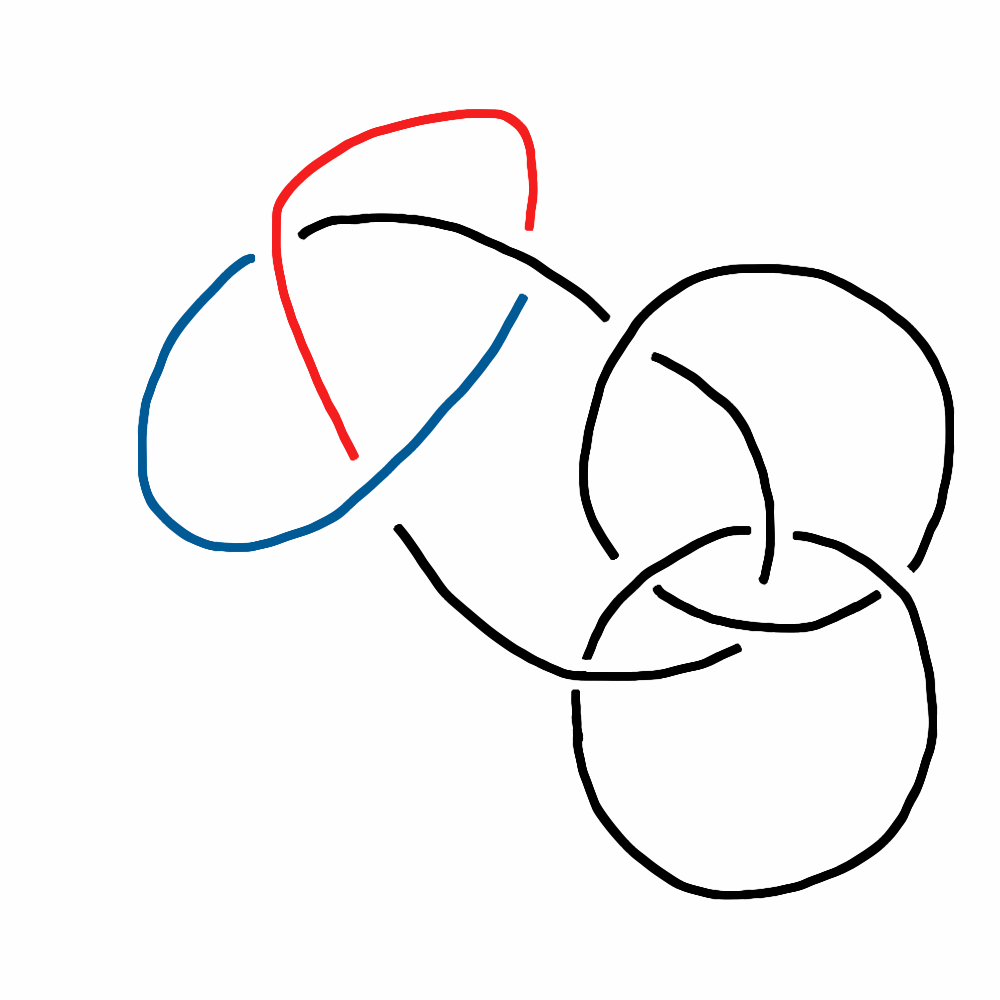
\includegraphics[width=.3\textwidth]{knotpics/borromean-trefoil-tricolor.png}
        \caption{Link E tricolored}
\end{figure}

Also, links A and B are equivalent by an ambient isotopy. This can be realized with a short series of Reidemeister moves, as shown here:

\begin{figure}[h]
    \centering
        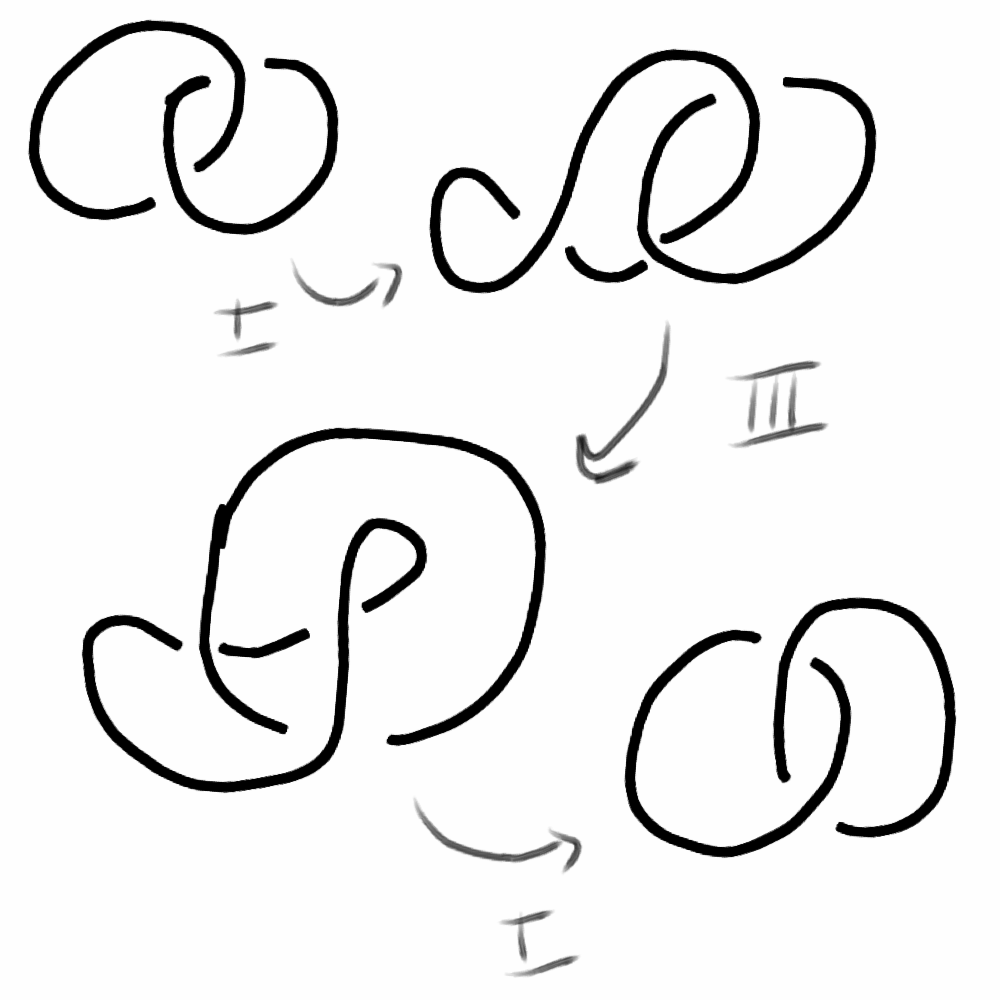
\includegraphics[width=.4\textwidth]{knotpics/hopf-rm-mirror.png}
        \caption{Reidemeister moves from link A to link B}
\end{figure}

\end{document}